\chapter{Architektura systemu}
W tym rozdziale opisana zostanie architektura systemu. Przedstawione zostaną główne elementy składowe systemu oraz ich interakcje. 

\section{Identyfikacja aktorów}
Biorąc pod uwagę założenia opisane w poprzednich podrozdziałach, zaprojektowany został diagram przypadków użycia aplikacji. Idnetyfikacja aktorów:
\begin{enumerate}
\item Użytkownik - ogólny użytkownik systemu. Reprezentuje dowolną osobę korzystającą z serwisu, jego przypadki użycia będą dziedziczone przez pozostałych aktorów systemu.
\begin{figure}[H]
	\centering
		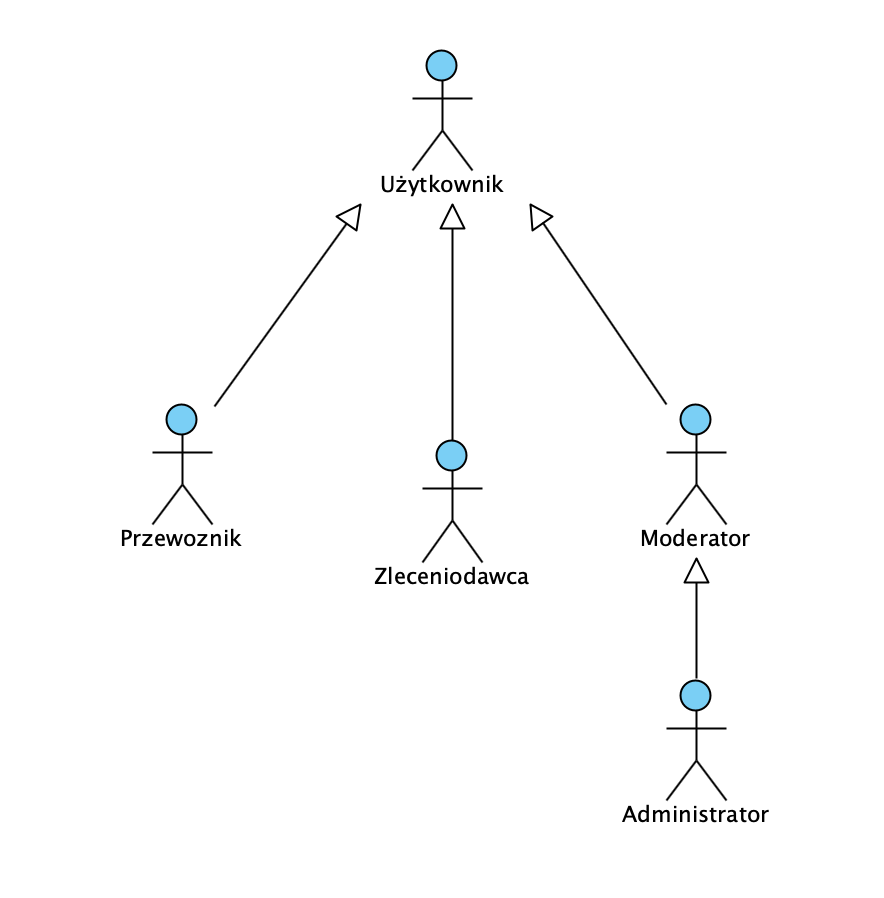
\includegraphics[width=0.6\linewidth]{rozdzial1/dziedziczenie.png}
	\caption{Graficzne ukazanie dziedziczenia możliwości aktorów}
	\label{Rys. fig:Graficzne ukazanie dziedziczenia możliwości aktorów}
\end{figure}
\item Przewoźnik - aktor odpowiedzialny za transport towarów. Może przeglądać dostępne zlecenia, dodawać ogłoszenia o planowanych trasach, komunikować się z autorami ogłoszeń, przyjmować zlecenia oraz oceniać i komentować kontrahentów.
\item Zleceniodawca - użytkownik systemu, który zleca transport towarów. Może dodawać nowe zlecenia transportowe, podobnie jak przewoźnik, może również przeglądać ogłoszenia przewoźników oraz komunikować się z autorami ogłoszeń.
\item Moderator - osoba odpowiedzialna za zarządzanie systemem. Moderator zatwierdza lub usuwa nowe ogłoszenia i zlecenia oraz blokuje konta użytkowników.
\item Administrator - użytkownik umiejscowiony najwyżej w hierarchii systemu. Może on wykonywać wszystko co moderator, lecz ma również możliwość dodawania nowych moderatorów lub usuwania obecnych.
\end{enumerate}

\section{Przypadki użycia}
W tej sekcji przedstawione zostaną diagramy przypadków użycia serwisu \texttt{CargoLink}, korzystając z definicji aktorów opisanych powyżej.
\begin{figure}[H]
	\centering
		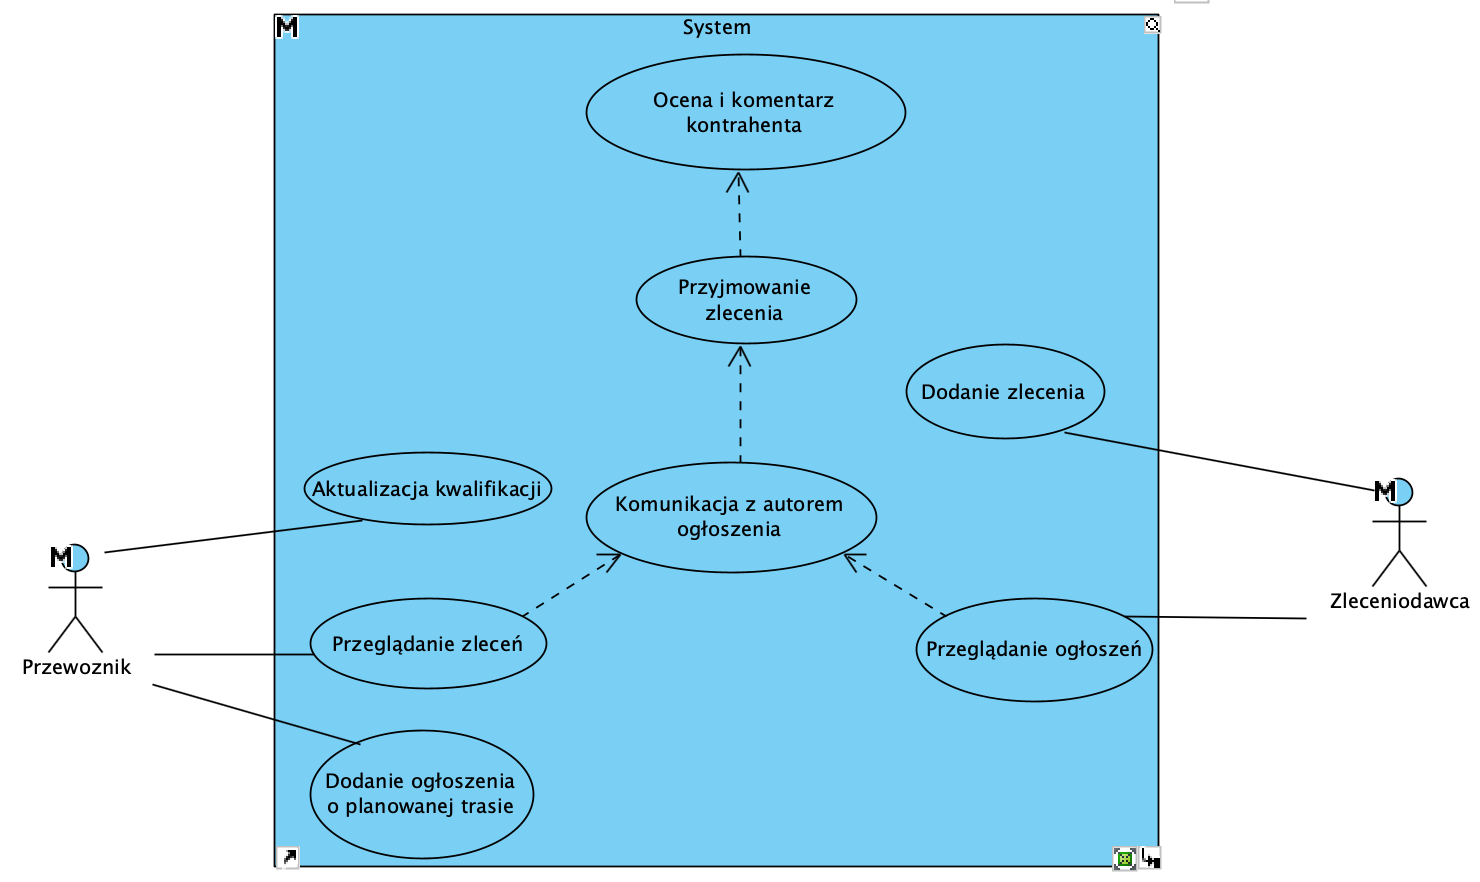
\includegraphics[width=0.9\linewidth]{rozdzial1/glowne_zalozenia.png}
	\caption{Diagram głównych funkcjonalności aplikacji}
	\label{Rys. fig:Diagram głównych funkcjonalności aplikacji}
\end{figure}

Na powyższym obrazku przedstawiony został diagram przypadków użycia dla przewoźnika oraz zleceniodawcy.

\begin{figure}[H]
	\centering
		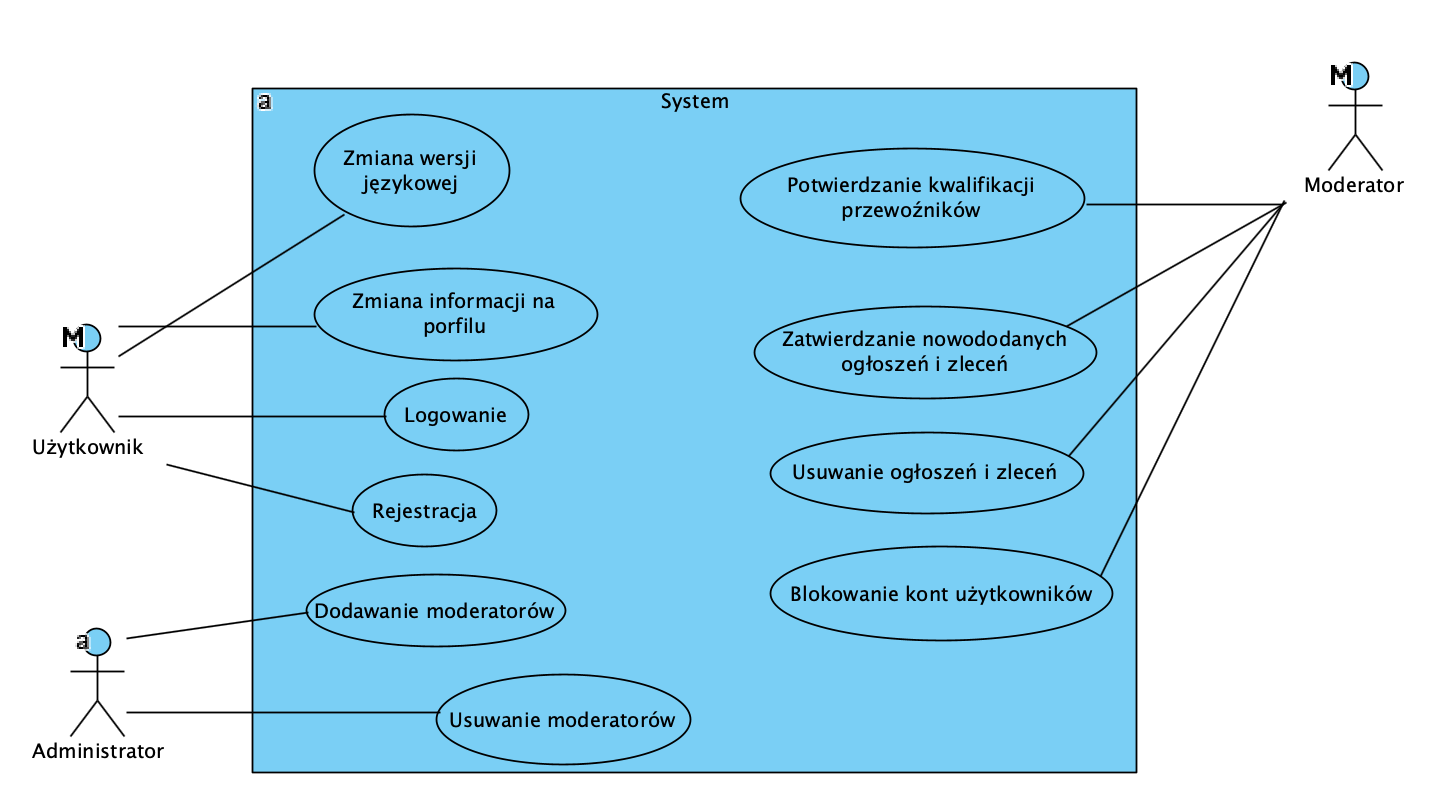
\includegraphics[width=0.9\linewidth]{rozdzial1/ogolny_schemat.png}
	\caption{Główne założenia projektowe od strony zarządzania serwisem}
	\label{Rys. fig:Główne założenia projektowe od strony zarządzania serwisem}
\end{figure}

Diagram ukazujący główne założenia systemu od strony zarządzania serwisem, w tym możliwości użytkownika, moderatora oraz administratora.
